\documentclass{beamer}
\mode<presentation>
\usetheme{CambridgeUS}
\usepackage[russian]{babel}
\usepackage[utf8]{inputenc}
\usepackage[T2A]{fontenc}
\usepackage{sansmathaccent}

\usepackage{verbatim}
\usepackage{alltt}

\pdfmapfile{+sansmathaccent.map}
\title[Artifical Intelligence]{Регрессия}
\author{Наумов Д.А., доц. каф. КТ}
\date[11.03.2020] {Экспертные системы и искусственный интеллект, 2020}

\begin{document}

%ТИТУЛЬНЫЙ СЛАЙД
\begin{frame}
  \titlepage
\end{frame}
  
%СОДЕРЖАНИЕ ЛЕКЦИИ
\begin{frame}
  \frametitle{Содержание лекции}
  \tableofcontents  
\end{frame}

\section{Машинное обечение и библиотека Scikit-Learning}

\begin{frame}{Машинное обучение}
\begin{block}{Машинное обучение, Mashine Learning, ML}
часть сферы искусственного интеллекта, средство построения математических моделей для исследования данных.
\end{block}
Задачи ML:
\begin{itemize}
\item этап обучения - определение настраиваемых параметров модели, которые нужно "приспособить" для отражения наблюдаемых данных;
\item использование модели для предсказания и понимания различных аспектов данных новых наблюдений.
\end{itemize}
\begin{block}{Категории машинного обучения}
\begin{itemize}
\item обучение с учителем (supervised learning) - классификация, регрессия;
\item обучение без учителя (supervised learning) - кластеризация, понижение размерности.
\end{itemize}
\end{block}
\end{frame}

\begin{frame}{Библиотека Scikit-Learn}
Библиотека Scikit-Learn:
\begin{itemize}
\item пакет, предоставляющий эффективные версии множества распространенных алгоритмов;
\item единообразный API, позволяющий легко перейти от одной модели к другой.
\begin{itemize}
\item представление данных (data representation);
\item применение API статистического оценивания (API Estimator).
\end{itemize}
\end{itemize}
\end{frame}

\begin{frame}{Библиотека Scikit-Learn}
\begin{figure}[h]
\centering
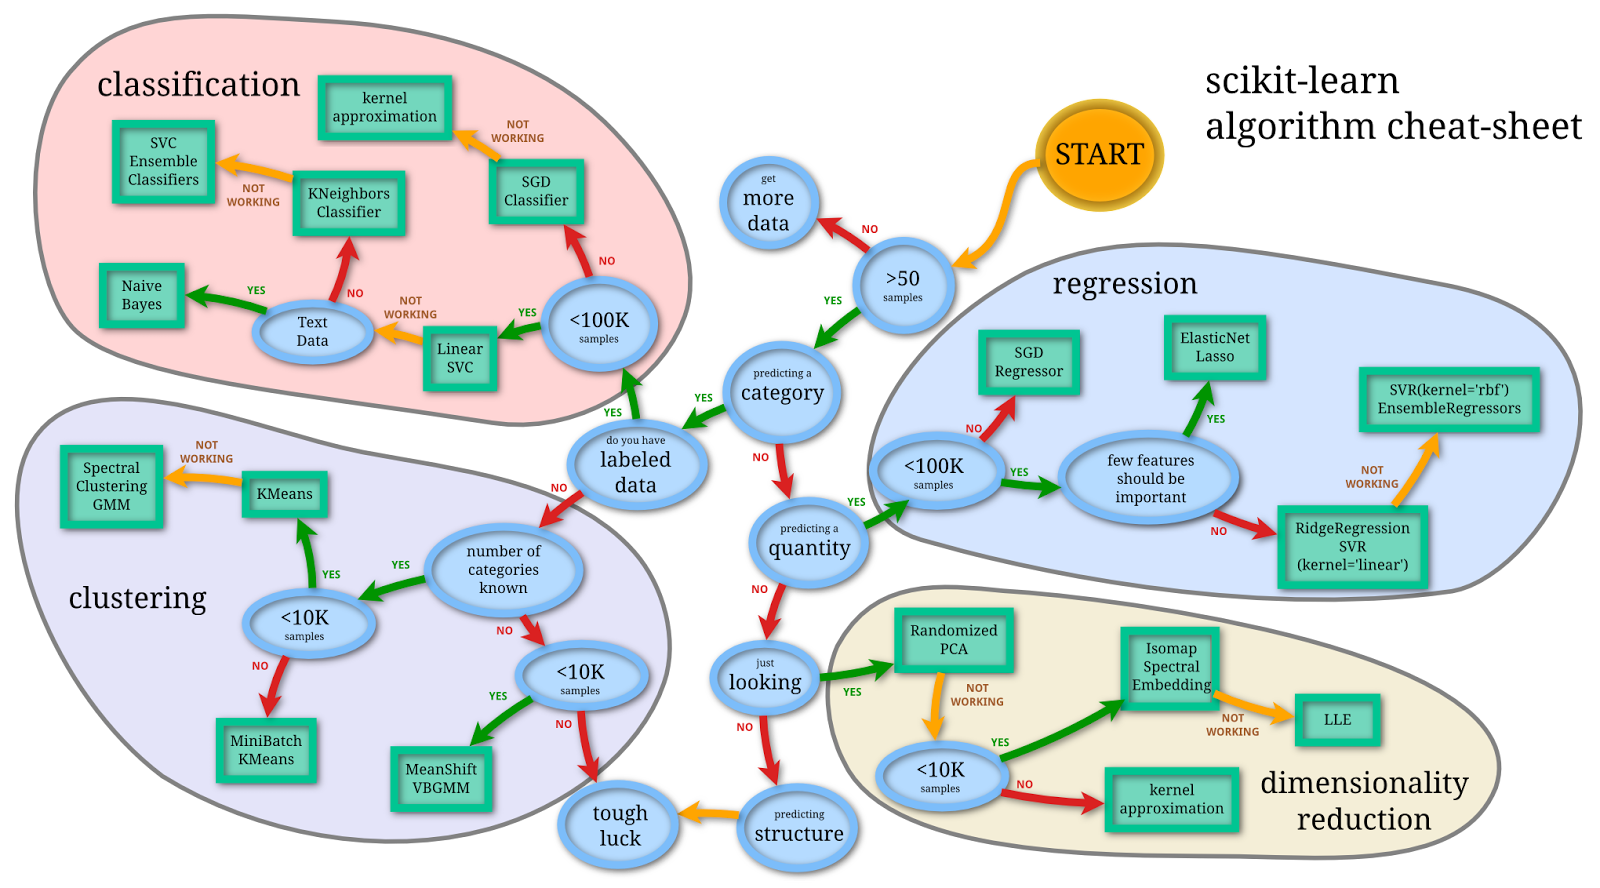
\includegraphics[scale=0.2]{images/scikit.png}
\end{figure}
\end{frame}

\begin{frame}
\begin{block}{Основное представление - таблица}
двумерная сетка данных, в которой строки представляют отдельные элементы набора данных, а столбцы — атрибуты, связанные с каждым из этих элементов.
\end{block}
\begin{figure}[h]
\centering
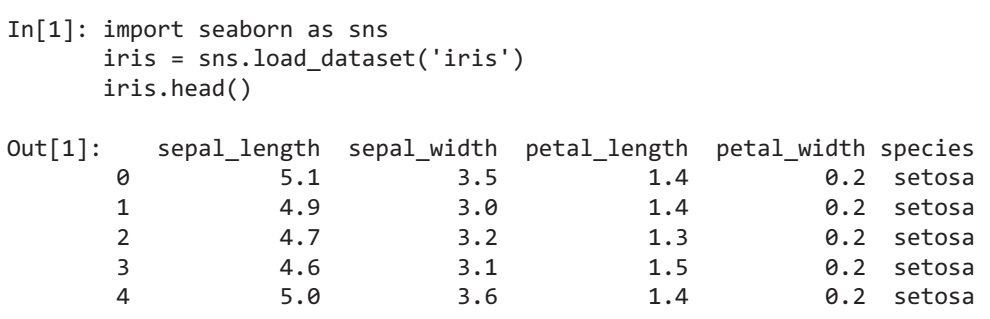
\includegraphics[scale=0.4]{images/lec10-pic01.png}
\end{figure}
\begin{itemize}
\item строки - выборка (samples), соответствуют объектам;
\item столбцы - признаки (features), соотвествуют свойствами объектов.
\end{itemize}
\end{frame}

\begin{frame}
Принятые обозначения:
\begin{itemize}
\item X[n\_samples, n\_features] - матрица признаков (features matrix); варианты представления: массив NumPy, Pandas.DataFrame, разреженная матрица SciPy.
\item y[n\_samples] - целевой массив принзнаков; величину, значения которой мы хотим предсказать на основе имеющихся данных. Варианты представления: массив NumPy, Pandas.Series.
\end{itemize}
\end{frame}

\section{Визуализация данных}

\begin{frame}[fragile]{Seaborn}
\begin{block}{Seaborn}
высокоуровневое API на базе библиотеки matplotlib, содержащее дефолтные настройки оформления графиков и сложные типы визуализации, которые в matplotlib потребовали бы большого количество кода.
\end{block}
Импортируем необходимые библиотеки и загрузим данные о продажах и оценках видео-игр из Kaggle Datasets.
\begin{alltt}
import seaborn as sns
import matplotlib.pyplot as plt
import pandas as pd
df = pd.read_csv('code/regression/video_games_sales.csv')
df.info()
\end{alltt}
\end{frame}

\begin{frame}[fragile]{Data}
Оставим только те записи, в которых нет пропусков, с помощью метода dropna.
\begin{alltt}
df = df.dropna()
print(df.shape)
\end{alltt}
Посмотрим на несколько первых записей c помощью метода head. 
\begin{alltt}
useful_cols = ['Name', 'Platform', 'Year_of_Release', 'Genre', 
               'Global_Sales', 'Critic_Score', 'Critic_Count',
               'User_Score', 'User_Count', 'Rating'
              ]
df[useful_cols].head()
\end{alltt}
\begin{figure}[h]
\centering
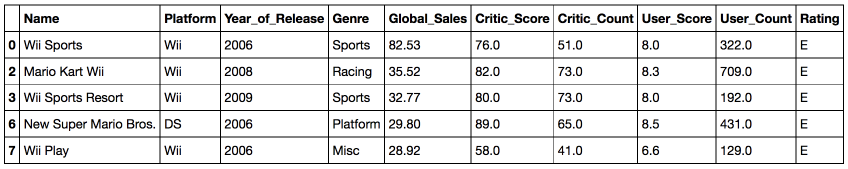
\includegraphics[scale=0.3]{images/seaborn-01.png}
\end{figure}
\end{frame}

\begin{frame}[fragile]{Plot}
Воспользуемся функцией plot - построим график продаж видео игр в различных странах в зависимости от года. 
\begin{alltt}
sales_df = df[[x for x in df.columns if 'Sales' in x] + ['Year_of_Release']]
sales_df.groupby('Year_of_Release').sum().plot()
\end{alltt}
\begin{figure}[h]
\centering
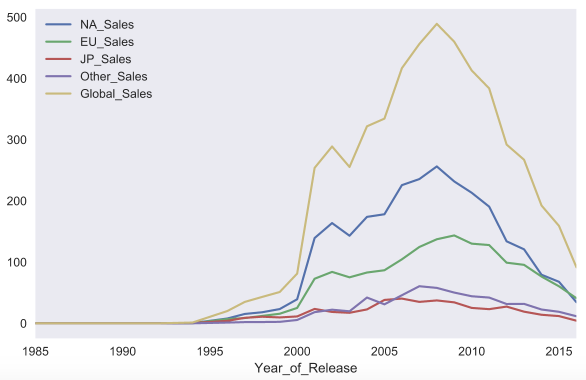
\includegraphics[scale=0.4]{images/seaborn-02.png}
\end{figure}
\end{frame}

\begin{frame}[fragile]{Plot}
C помощью параметра kind можно изменить тип графика, например, на bar chart. 
\begin{alltt}
sales_df.groupby('Year_of_Release').sum().plot(kind='bar', rot=45)
\end{alltt}
\begin{figure}[h]
\centering
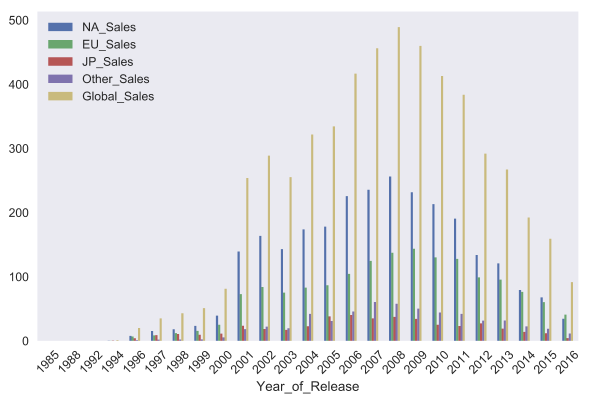
\includegraphics[scale=0.4]{images/seaborn-03.png}
\end{figure}
\end{frame}

\begin{frame}[fragile]
Графики типа pair plot (scatter plot matrix) позволяет посмотреть на одной картинке, как связаны между собой различные признаки. 
\begin{alltt}
cols = ['Global_Sales', 'Critic_Score', 'Critic_Count', 'User_Score', 'User_Count']
sns_plot = sns.pairplot(df[cols])
sns_plot.savefig('pairplot.png')
\end{alltt}
\begin{figure}[h]
\centering
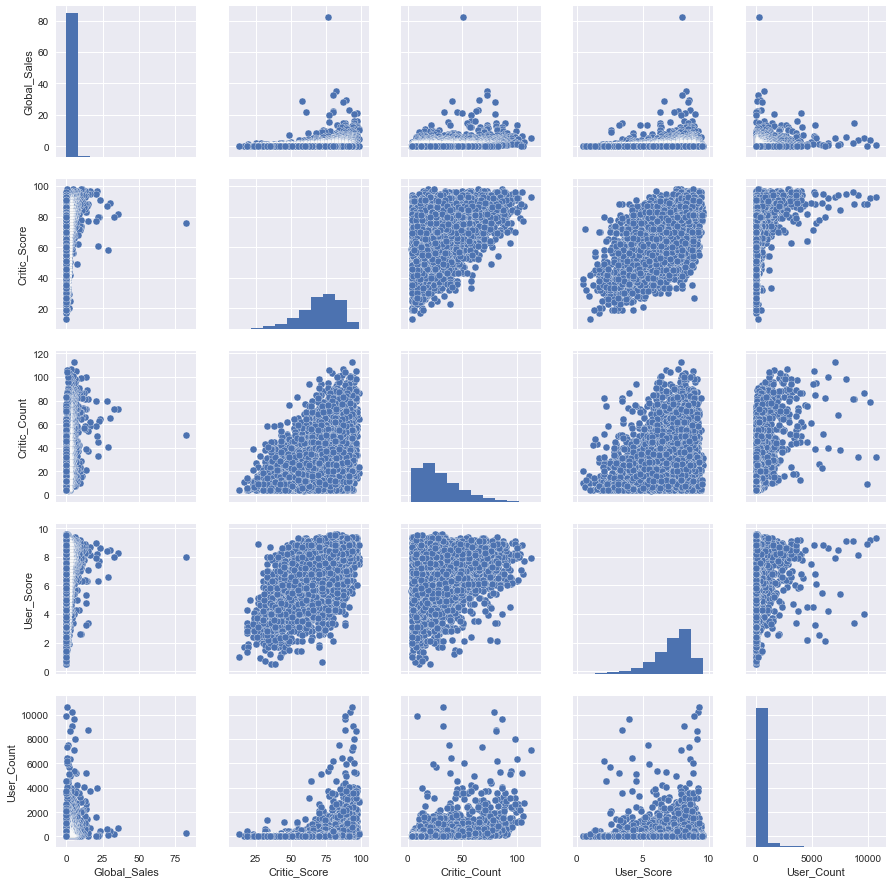
\includegraphics[scale=0.2]{images/seaborn-04.png}
\end{figure}
\end{frame}

\begin{frame}[fragile]
С помощью seaborn можно построить и распределение dist plot. Для примера посмотрим на распределение оценок критиков Critic\_Score. 
\begin{alltt}
sns.distplot(df.Critic_Score)
\end{alltt}
\begin{figure}[h]
\centering
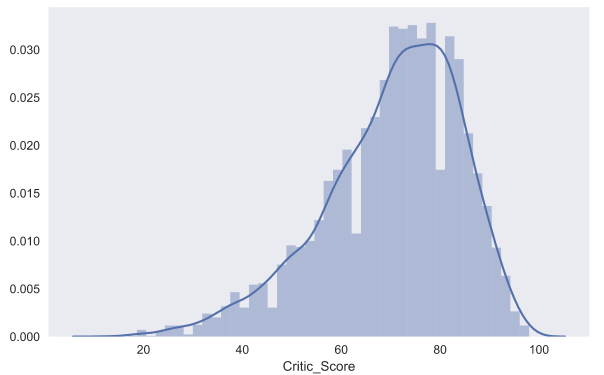
\includegraphics[scale=0.5]{images/seaborn-05.png}
\end{figure}
\end{frame}

\begin{frame}[fragile]
Для того, чтобы подробнее посмотреть на взаимосвязь двух численных признаков, есть joint plot — гибрид scatter plot и histogram.
\begin{alltt}
cols = ['Critic_Score', 'User_Score']
sns.jointplot(df[cols])
\end{alltt}
\begin{figure}[h]
\centering
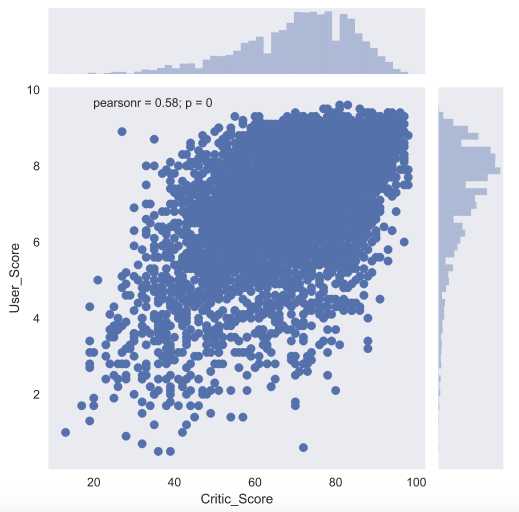
\includegraphics[scale=0.35]{images/seaborn-06.png}
\end{figure}
\end{frame}

\begin{frame}[fragile]
Cравним оценки игр от критиков для топ-5 крупнейших игровых платформ при помощи графиков box\_plot.
\begin{alltt}
top\_platforms = df.Platform.value_counts().sort\_values(
    ascending = False).head(5).index.values
sns.boxplot(y="Platform", x="Critic\_Score", 
    data=df[df.Platform.isin(top\_platforms)], orient="h")
\end{alltt}
\begin{figure}[h]
\centering
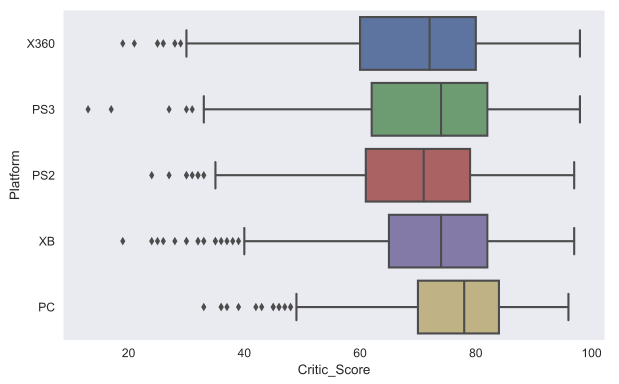
\includegraphics[scale=0.35]{images/seaborn-07.png}
\end{figure}
\end{frame}

\begin{frame}[fragile]
\begin{figure}[h]
\centering
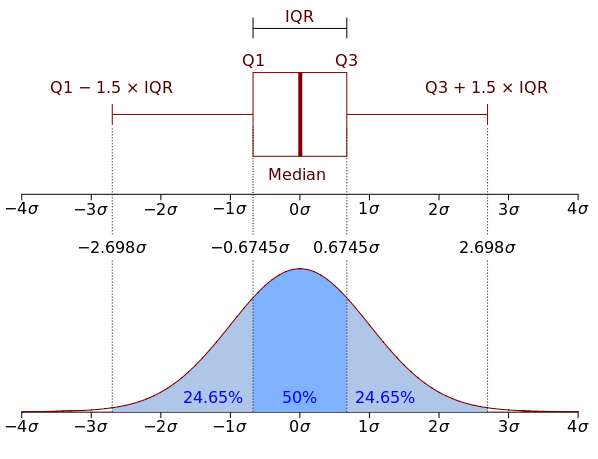
\includegraphics[scale=0.6]{images/seaborn-08.png}
\end{figure}
\end{frame}

\begin{frame}[fragile]
Heat map позволяет посмотреть на распределение какого-то численного признака по двум категориальным. Визуализируем суммарные продажи игр по жанрам и игровым платформам.
\begin{alltt}
platform_genre_sales = df.pivot_table(
                        index='Platform', 
                        columns='Genre', 
                        values='Global_Sales', 
                        aggfunc=sum).fillna(0).applymap(float)
sns.heatmap(platform_genre_sales, annot=True, fmt=".1f", linewidths=.5)
\end{alltt}
\begin{figure}[h]
\centering
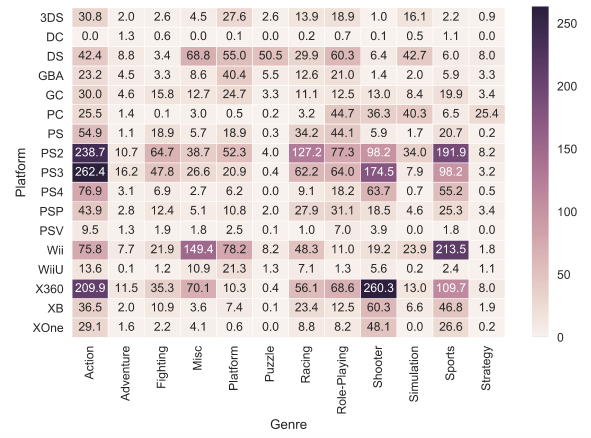
\includegraphics[scale=0.25]{images/seaborn-09.png}
\end{figure}
\end{frame}

\begin{frame}{API Scikit-Learn}
Использование API статистического оценивания:
\begin{enumerate}
\item Выбор класса модели с помощью импорта соответствующего класса оценивателя из библиотеки Scikit-Learn.
\item Выбор гиперпараметров модели путем создания экземпляра этого класса с соответствующими значениями.
\item Компоновка данных в матрицу признаков и целевой вектор в соответствии
с описанным выше.
\item Обучение модели на своих данных посредством вызова метода fit() экземпляра
модели.
\item Применение модели к новым данным (в случае машинного обучения с учителем метки для неизвестных данных обычно предсказывают с помощью метода predict()).
\end{enumerate}
\end{frame}

\section{Линейная регрессия}

\begin{frame}
\begin{block}{Линейная регрессия}
модель зависимости объясняемой переменной $y$ от объясняющих ее факторов, причем функция зависимости является линейной:
\[y = w_0 + \sum\limits_{i=0}^n{w_i x_i} \]
\end{block}
Зададим модель следующим образом:
\[\vec{y} = X\vec{w}+\epsilon\]
\begin{itemize}
\item $\vec{y}\in R^n$ - объясняемая (или целевая) переменная;
\item $w$ - вектор параметров модели (веса модели);
\item $X$ - матрица наблюдений и признаков размерности $n$ строк на $m+1$ столбцов (включая фиктивную единичную колонку слева);
\item $\epsilon$ -  случайная переменная, соответствующая случайной, непрогнозируемой ошибке модели.
\end{itemize}
\end{frame}

\begin{frame}{Линейная регрессия}
Ограничения на модель:
\begin{itemize}
\item матожидание случайных ошибок равно нулю;
\item дисперсия случайных ошибок одинакова и конечна (гомоскедастичность);
\item случайные ошибки не скоррелированы.
\end{itemize}
Пример графика остатков в случае простой линейной зависимости:
\begin{figure}[h]
\centering
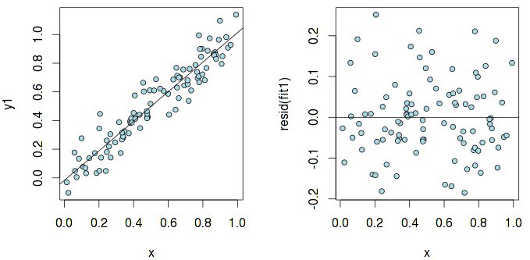
\includegraphics[scale=0.4]{images/error-01.png}
\end{figure}
Остатки равномерно распределены относительно горизонтальной оси.
\end{frame}

\begin{frame}{Линейная регрессия}
Исследуем график, но построенный для линейной модели (для данных, которые на самом деле не является линейными):
\begin{figure}[h]
\centering
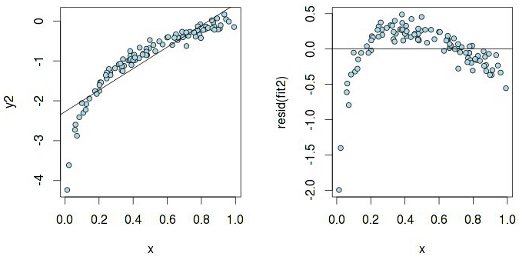
\includegraphics[scale=0.5]{images/error-02.png}
\end{figure}
По графику $y(x)$ бы можно предположить линейную зависимость, но у остатков есть паттерн, а значит, чистая линейная регрессия тут не пройдет. 
\end{frame}

\begin{frame}{Линейная регрессия}
Пример не гетероскедастичности:
\begin{figure}[h]
\centering
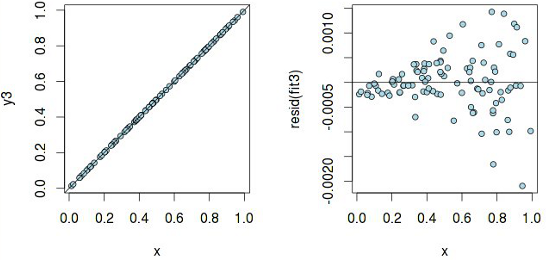
\includegraphics[scale=0.5]{images/error-03.png}
\end{figure}
Линейная модель с такими "раздувающимися" остатками не будет корректна. 
\end{frame}

\begin{frame}{Линейная регрессия}
Пример выброса (резко выделяющегося значения):
\begin{figure}[h]
\centering
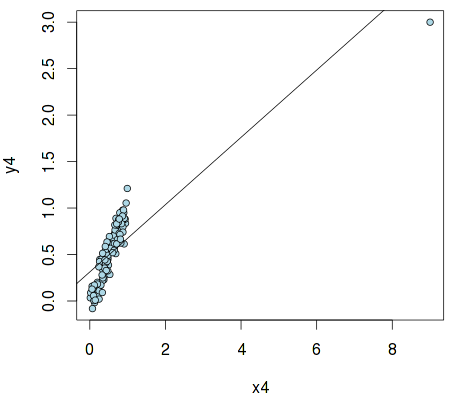
\includegraphics[scale=0.4]{images/error-04.png}
\end{figure}
Выброс который может сильно исказить результаты и привести к ошибочным выводам.
\end{frame}

\begin{frame}[fragile]{Пример: линейная регрессия}
Построим простую линейную регрессию - часто встречающийся случай подбора аппроксимирующей прямой для данных вида (x, y):
\begin{figure}[h]
\centering
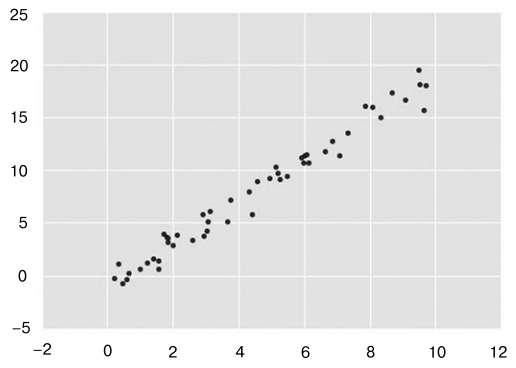
\includegraphics[scale=0.3]{images/ex-01-01.png}
\end{figure}
\begin{alltt}
import matplotlib.pyplot as plt
import numpy as np
rng = np.random.RandomState(42)
x = 10 * rng.rand(50)
y = 2 * x - 1 + rng.randn(50)
plt.scatter(x, y)
\end{alltt}
\end{frame}

\begin{frame}[fragile]{Пример: линейная регрессия}
\begin{block}{1. Выбор класса модели}
Каждый класс модели в Scikit-Learn представлен соответствующим классом языка Python. 
\begin{alltt}
from sklearn.linear_model import LinearRegression
\end{alltt}
\end{block}
\begin{block}{2. Выбор гиперпараметров модели}
\begin{itemize}
\item Хотим ли мы выполнить подбор сдвига прямой?
\item Хотим ли мы нормализовать модель?
\item Хотим ли мы сделать модель более гибкой, выполнив предварительную обработку признаков?
\item Какая степень регуляризации должна быть у нашей модели?
\item Сколько компонент модели мы хотели бы использовать?
\end{itemize}
\end{block}
\end{frame}

\begin{frame}[fragile]{Пример: линейная регрессия}
\begin{block}{2. Выбор гиперпараметров модели}
Создадим экземпляр класса LinearRegression и укажем с помощью гиперпараметра fit\_intercept, что нам бы хотелось выполнить подбор точки пересечения с осью координат:
\begin{alltt}
model = LinearRegression(fit\_intercept=True)
\end{alltt}
API Scikit-Learn разделяет выбор модели и применение модели к данным.
\end{block}
\begin{block}{3. Формирование из данных матриц признаков и целевого вектора}
Измененим форму одномерного массива X, чтобы привести ее к размерности [n\_samples, n\_features]:
\begin{alltt}
X = x[:, np.newaxis]
X.shape
\end{alltt}
\end{block}
\end{frame}

\begin{frame}[fragile]{Пример: линейная регрессия}
\begin{block}{4. Обучение модели на данных}
Применим модель к данным с помощью метода fit() модели:
\begin{alltt}
model.fit(X, y)
\end{alltt}
Команда fit() вызывает выполнение множества вычислений, в зависимости от модели, и сохранение результатов этих вычислений в атрибутах модели, доступных для просмотра пользователем:
\begin{alltt}
print('coef = ', model.coef\_)
print('intercept = ', model.intercept\_)
\end{alltt}
Эти два параметра представляют собой угловой коэффициент и точку пересечения с осью координат для простой линейной аппроксимации наших данных.
\end{block}
\end{frame}

\begin{frame}[fragile]{Пример: линейная регрессия}
\begin{block}{5. Предсказание новых значений}
После обучения модели главная задача машинного обучения с учителем заключается в вычислении с ее помощью значений для новых данных, не являющихся
частью обучающей последовательности:
\begin{alltt}
xfit = np.linspace(-1, 11)
\end{alltt}
Как и ранее, эти x-значения требуется преобразовать в матрицу признаков
[n\_samples, n\_features], после чего можно подать их на вход модели:
\begin{alltt}
Xfit = xfit[:, np.newaxis]
yfit = model.predict(Xfit)
\end{alltt}
\end{block}
\end{frame}

\begin{frame}[fragile]{Пример: линейная регрессия}
\begin{block}{5. Предсказание новых значений}
Визуализируем результаты, нарисовав сначала график исходных данных, а затем обученную модель:
\begin{alltt}
plt.scatter(x, y)
plt.plot(xfit, yfit)
\end{alltt}
\end{block}
\begin{figure}[h]
\centering
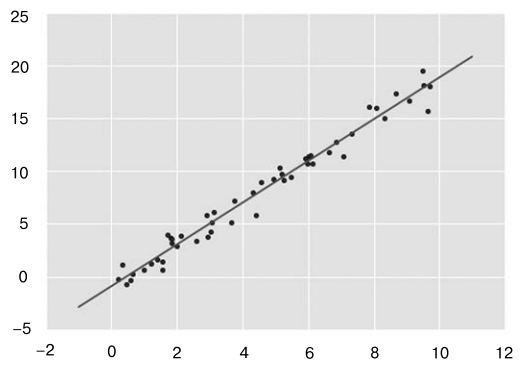
\includegraphics[scale=0.4]{images/ex-01-02.png}
\end{figure}
\end{frame}

\section{Комбинация базисных функций}

\begin{frame}[fragile]
\begin{block}{Комбинация базисных функций}
позволяет приспособить линейную регрессию к нелинейным отношениям между переменными, путем преобразования данных в соответствии базисными функциями. 
\end{block}
За основу берется многомерная линейную модель:
\[y = a_0+a_1x_1+a_2x_2+a_3x_3...\]
$x_1, x_2, x_3$ получаются на основе имеющегося одномерного входного значения $x_n=F_n(x)$.

Например, если $x_n = x^n$, то модель превращается в полиномиальную регрессию:
\[y = a_0+a_1x^1+a_2x^2+a_3x^3...\]
\begin{itemize}
\item модель по-прежнему остается линейной - коэффициенты $a_n$ не умножаются и не делятся друг на друга;
\item мы взяли одномерные значения x и выполнили проекцию их на более многомерное пространство.
\end{itemize}
\end{frame}

\begin{frame}[fragile]{Полиномиальные базисные функции}
Полиномиальная проекция встроена в библиотеку Scikit-Learn в виде преобразователя PolynomialFeatures:
\begin{alltt}
from sklearn.preprocessing import PolynomialFeatures
x = np.array([2, 3, 4])
poly = PolynomialFeatures(3, include_bias=False)
poly.fit_transform(x[:, None])
\end{alltt}
Преобразователь превратит одномерный массив в трехмерный путем возведения каждого из значений в степень:
\begin{alltt}
array([[ 2., 4., 8.],
[ 3., 9., 27.],
[ 4., 16., 64.]])
\end{alltt}
\end{frame}

\begin{frame}[fragile]{Полиномиальные базисные функции}
Создадим полиномиальную модель седьмого порядка:
\begin{alltt}
from sklearn.pipeline import make_pipeline
poly_model = make_pipeline(PolynomialFeatures(7), LinearRegression())
\end{alltt}
После такого преобразования можно воспользоваться линейной моделью для подбора намного более сложных зависимостей между величинами x и y:
\begin{alltt}
rng = np.random.RandomState(1)
x = 10 * rng.rand(50)
y = np.sin(x) + 0.1 * rng.randn(50)
poly_model.fit(x[:, np.newaxis], y)
xfit = np.linspace(0, 10, 1000)
yfit = poly_model.predict(xfit[:, np.newaxis])
plt.scatter(x, y)
plt.plot(xfit, yfit);
\end{alltt}
\end{frame}

\begin{frame}[fragile]{Полиномиальные базисные функции}
\begin{figure}[h]
\centering
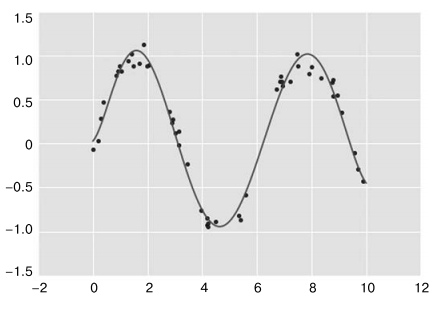
\includegraphics[scale=0.7]{images/polynom-01.png}
\end{figure}
С помощью линейной модели, используя полиномиальные базисные функции седьмого порядка, получена аппроксимацию этих нелинейных данных.
\end{frame}

\begin{frame}[fragile]{Гауссовы базисные функции}
Один из полезных паттернов - обучение модели, представляющей собой сумму не полиномиальных, а Гауссовых базисных функций:
\begin{figure}[h]
\centering
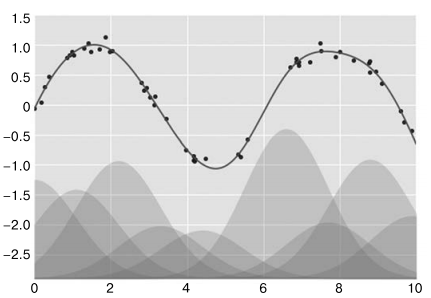
\includegraphics[scale=0.65]{images/gauss-01.png}
\end{figure}
Затененные области - нормированные базисные функции, дающие при сложении аппроксимирующую данные гладкую кривую.
\end{frame}

\begin{frame}[fragile]{Гауссовы базисные функции}
Гауссовы базисные функции не встроены в библиотеку Scikit-Learn, но можyj написать для их создания пользовательский преобразователь, как показано в примере (gauss.py):
\begin{figure}[h]
\centering
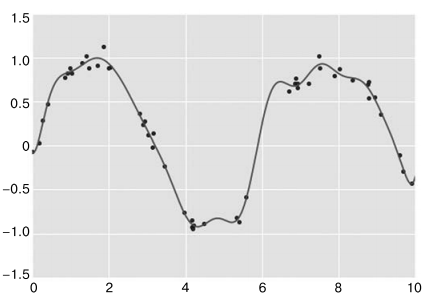
\includegraphics[scale=0.65]{images/gauss-02.png}
\end{figure}
\end{frame}

\section{Разложение ошибки на смещение и разброс}

\begin{frame}[fragile]{Разложение ошибки на смещение и разброс (Bias-variance decomposition)}
Ошибка прогноза любой модели вида $y=f(\vec{x}+\epsilon)$ складывается из:
\begin{itemize}
\item квадрата смещения $Bias(\hat{f})$ - средняя ошибка по всевозможным наборам данных;
\item дисперсии $Var(\hat{f})$ – вариативность ошибки, то, на сколько ошибка будет отличаться, если обучать модель на разных наборах данных;
\item неустранимой ошибки $\sigma^2$.
\end{itemize}
В идеале, конечно же, хотелось бы свести на нет оба этих слагаемых (левый верхний квадрат рисунка), но на практике часто приходится балансировать между смещенными и нестабильными оценками (высокая дисперсия).
\end{frame}

\begin{frame}[fragile]{Bias-variance decomposition}
\begin{figure}[h]
\centering
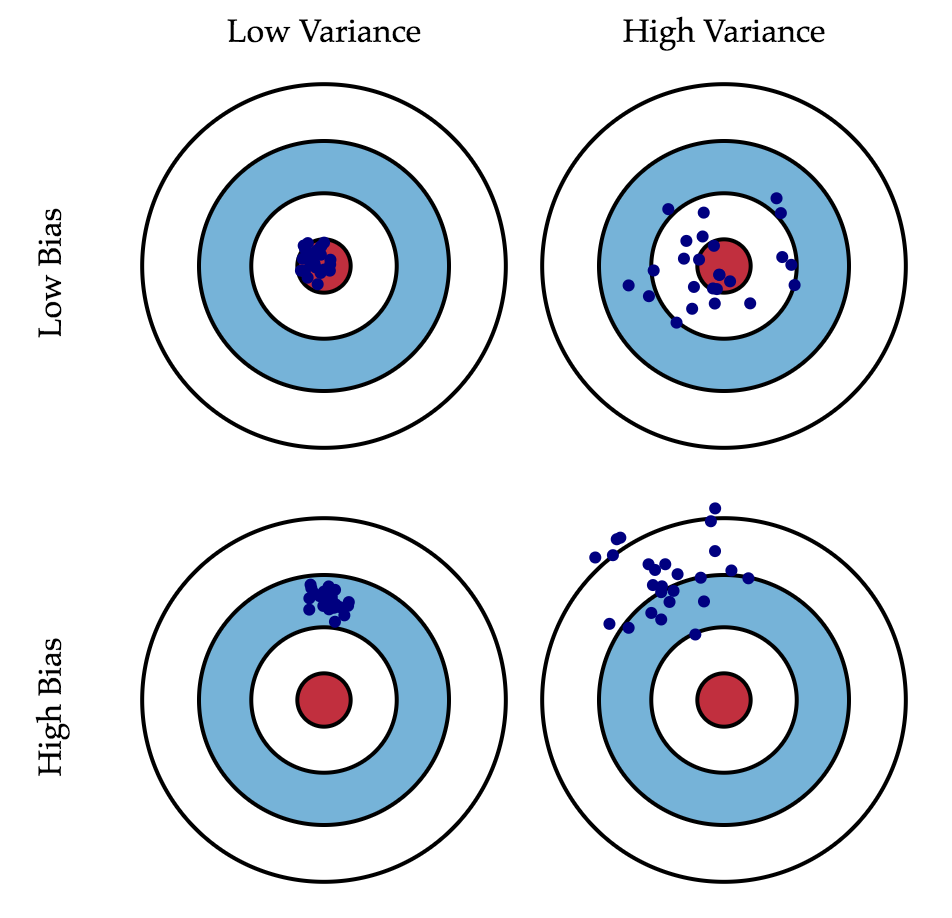
\includegraphics[scale=0.2]{images/bias-variant.png}
\end{figure}
При увеличении сложности модели (например, при увеличении количества свободных параметров) увеличивается дисперсия (разброс) оценки, но уменьшается смещение.
\end{frame}

\begin{frame}[fragile]{Bias-variance decomposition}
\begin{figure}[h]
\centering
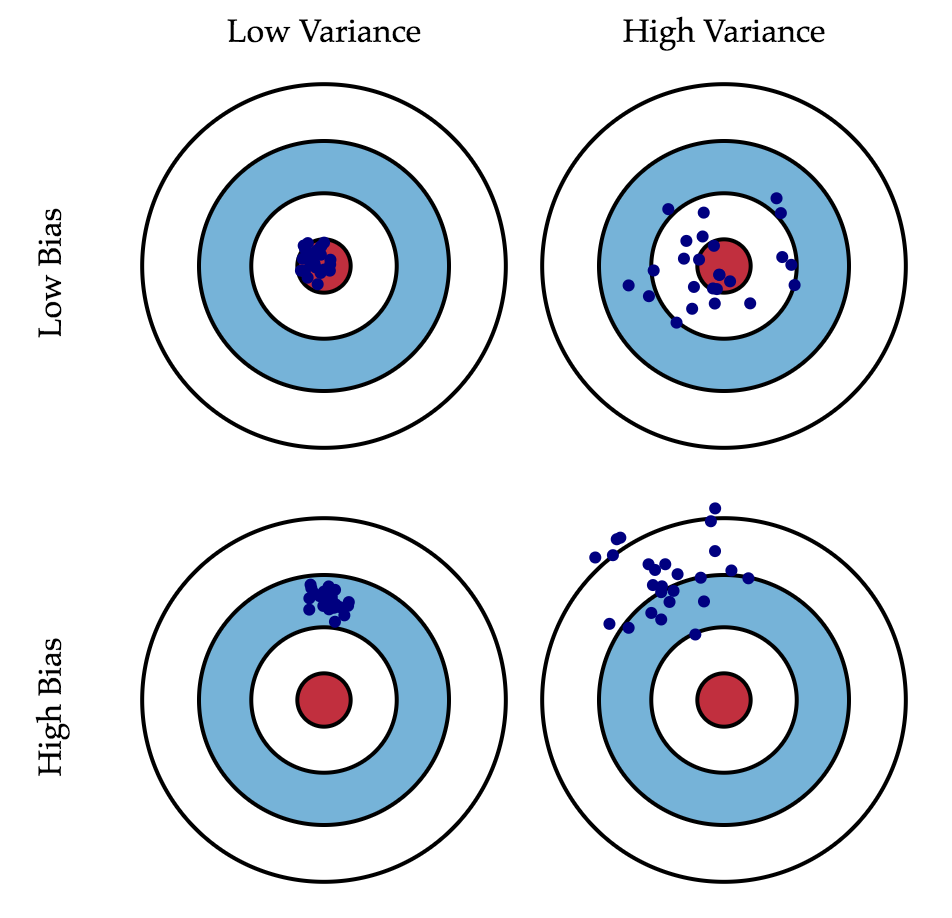
\includegraphics[scale=0.2]{images/bias-variant.png}
\end{figure}
\end{frame}

\section{Переобучение. Недообучение}

\begin{frame}[fragile]{Переобучение. Недообучение}
\begin{figure}[h]
\centering
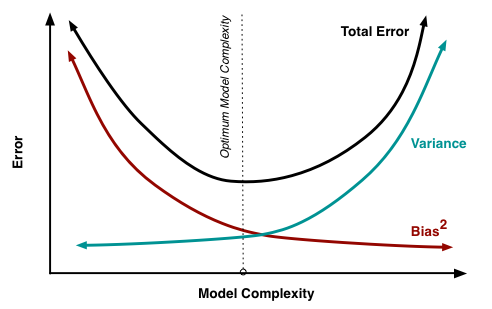
\includegraphics[scale=0.4]{images/complexity.png}
\end{figure}
\begin{itemize}
\item В сложной модели тренировочный набор данных полностью запоминается вместо обобщения, небольшие изменения приводят к неожиданным результатам (\textbf{переобучение}). 
\item Если же модель слабая, то она не в состоянии выучить закономерность, в результате выучивается что-то другое, смещенное относительно правильного решения (\textbf{недообучение}).
\end{itemize}
\end{frame}

\begin{frame}[fragile]{Переобучение на Гауссовой модели}
Если выбрать слишком много Гауссовых базисных функций, мы в итоге получим не слишком
хорошие результаты.
\begin{figure}[h]
\centering
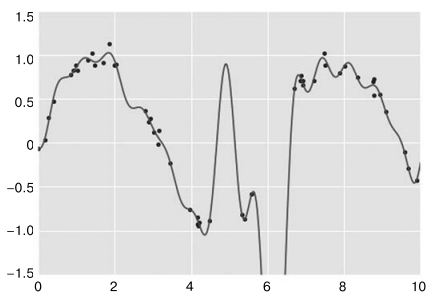
\includegraphics[scale=0.75]{images/complex-02.png}
\end{figure}
\end{frame}

\begin{frame}[fragile]
В результате проекции данных на 30-мерный базис модель оказалась слишком уж
гибкой и стремится к экстремальным значениям в промежутках между точками, в которых она ограничена данными.
\begin{figure}[h]
\centering
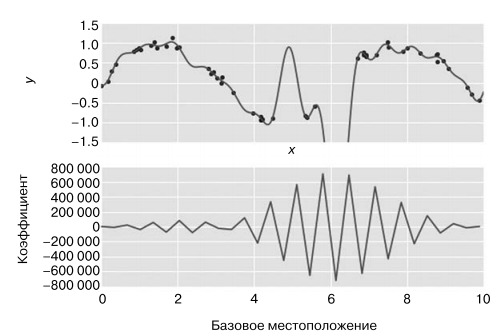
\includegraphics[scale=0.6]{images/complex-03.png}
\end{figure}
Причину этого можно понять, построив график коэффициентов Гауссовых базисных функций в соответствии с координатой x.
\end{frame}

\section{Линейный классификатор и логистическая регрессия}

\begin{frame}[fragile]{Линейный классификатор и логистическая регрессия}
Основная идея линейного классификатора заключается в том, что признаковое пространство может быть разделено гиперплоскостью на два полупространства, в каждом из которых прогнозируется одно из двух значений целевого класса.
\begin{figure}[h]
\centering
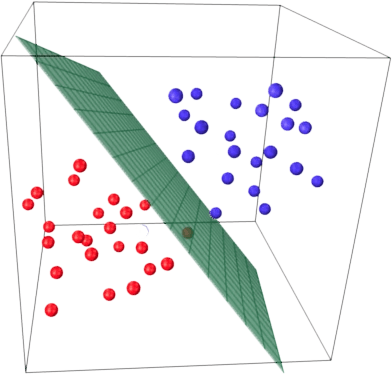
\includegraphics[scale=0.4]{images/logistic-01.png}
\end{figure}
Если это можно сделать без ошибок, то обучающая выборка называется линейно разделимой.
\end{frame}

\begin{frame}[fragile]{Логистическая регрессия}
Логистическая регрессия - задача бинарной классификации, причем метки целевого класса "+1" (положительные примеры) и "-1" (отрицательные примеры).
\begin{figure}[h]
\centering
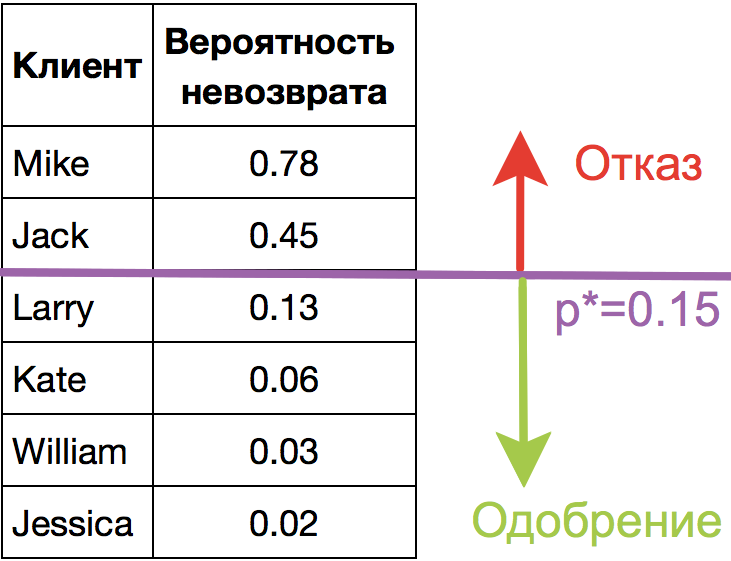
\includegraphics[scale=0.3]{images/logistic-02.png}
\end{figure}
\end{frame}

\begin{frame}[fragile]{Логистическая регрессия}
Для преобразования линейного прогноза $b(\vec{x})=\vec{w}^T\vec{x} \in R$ в вероятность отнесения к классу необходима функция $f: R\rightarrow[0,1]$.

В модели логистической регрессии берется функция 
\[\sigma(z)=\frac{1}{1+e^{-z}}\]
\begin{figure}[h]
\centering
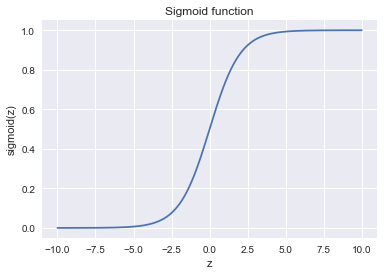
\includegraphics[scale=0.5]{images/sigmoid.png}
\end{figure}
\end{frame}

\section{Регуляризация}

\begin{frame}[fragile]{Регуляризация}
В задаче классификации, не умея напрямую минимизировать число ошибок, мы минимизируем некоторую ее верхнюю оценку, задаваемую \textbf{логистической функции потерь}.
\[\large \hat{w} = \arg \min_{\vec{w}} J(X, \vec{y}, \vec{w}) = \arg \min_{\vec{w}}\ (C\sum_{i=1}^{\ell} \log (1 + \exp^{-y_i\vec{w}^T\vec{x_i}})+ |\vec{w}|^2)\]
L2-регуляризация модели встроена в библиотеку Scikit-Learn в виде оценивателя Ridge.
\begin{alltt}
from sklearn.linear_model import Ridge
model = make_pipeline(GaussianFeatures(30), Ridge(alpha=0.1))
basis_plot(model, title='Ridge Regression')
\end{alltt}
\end{frame}

\begin{frame}[fragile]
Параметр $\alpha$ служит для управления сложностью получаемой в итоге модели.
\begin{figure}[h]
\centering
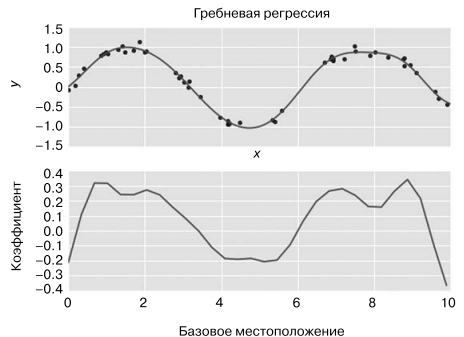
\includegraphics[scale=0.5]{images/logistic.png}
\end{figure}
\begin{itemize}
\item В предельном случае $\alpha \rightarrow 0$ мы получаем результат, соответствующий стандартной линейной регрессии; 
\item в предельном случае $\alpha \rightarrow \infty$ будет происходить подавление любого отклика модели. 
\end{itemize}
\end{frame}

\begin{frame}[fragile]{Пример. Регуляризация логистической регрессии}
\begin{itemize}
\item Посмотрим, как регуляризация влияет на качество классификации на наборе данных по тестированию микрочипов из курса Andrew Ng по машинному обучению.
\item Будем использовать логистическую регрессию с полиномиальными признаками и варьировать параметр регуляризации C.
\item Сначала посмотрим, как регуляризация влияет на разделяющую границу классификатора, интуитивно распознаем переобучение и недообучение.
\item Потом численно установим близкий к оптимальному параметр регуляризации с помощью кросс-валидации (cross-validation) и перебора по сетке (GridSearch).
\end{itemize}
\end{frame}

\begin{frame}[fragile]{Пример. Регуляризация логистической регрессии}
\begin{figure}[h]
\centering
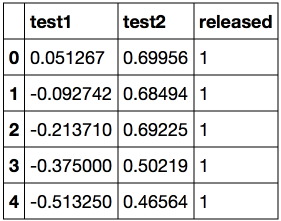
\includegraphics[scale=0.5]{images/test-01.png}
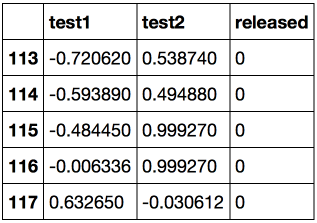
\includegraphics[scale=0.5]{images/test-02.png}
\end{figure}
\end{frame}

\begin{frame}[fragile]{Пример. Регуляризация логистической регрессии}
Сохраним обучающую выборку и метки целевого класса в отдельных массивах NumPy. Отобразим данные. Красный цвет соответствует бракованным чипам, зеленый – нормальным.
\begin{figure}[h]
\centering
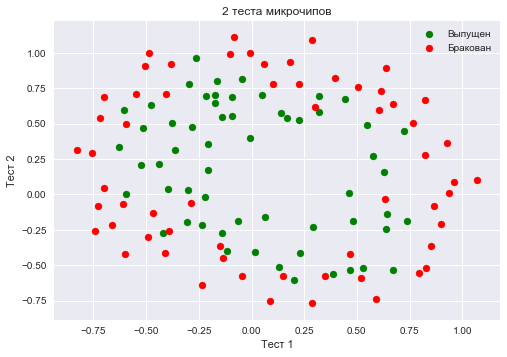
\includegraphics[scale=0.5]{images/test-03.png}
\end{figure}
\end{frame}

\begin{frame}[fragile]{Пример. Регуляризация логистической регрессии}
Сохраним обучающую выборку и метки целевого класса в отдельных массивах NumPy. Отобразим данные. Красный цвет соответствует бракованным чипам, зеленый – нормальным.
\begin{figure}[h]
\centering
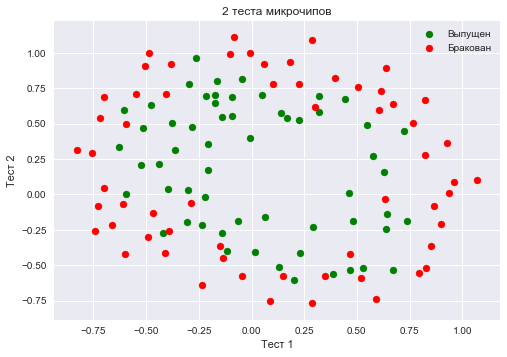
\includegraphics[scale=0.4]{images/test-03.png}
\end{figure}
\end{frame}

\begin{frame}[fragile]
Обучим логистическую регрессию с параметром регуляризации $C=10^{-2}$ c полиномами степени 7.
\begin{figure}[h]
\centering
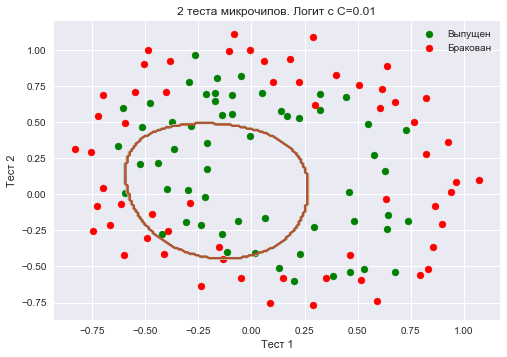
\includegraphics[scale=0.4]{images/test-04.png}
\end{figure}
Регуляризация оказалась слишком сильной, и модель "недообучилась". Доля правильных ответов классификатора на обучающей выборке оказалась равной 0.627.
\end{frame}

\begin{frame}[fragile]
Увеличим $C$ до 1. Тем самым мы ослабляем регуляризацию, теперь в решении значения весов логистической регрессии могут оказаться больше (по модулю), чем в прошлом случае.
\begin{figure}[h]
\centering
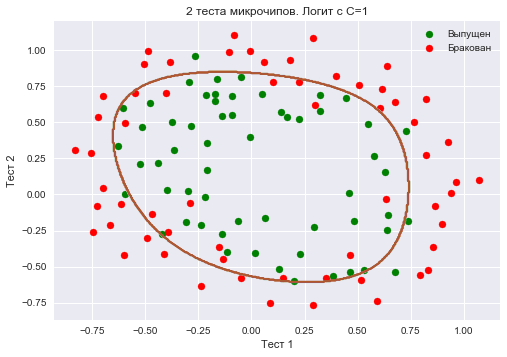
\includegraphics[scale=0.4]{images/test-05.png}
\end{figure}
Теперь доля правильных ответов классификатора на обучающей выборке – 0.831.
\end{frame}

\begin{frame}[fragile]
Еще увеличим  – до 10 тысяч. Теперь регуляризации явно недостаточно, и мы наблюдаем переобучение.
\begin{figure}[h]
\centering
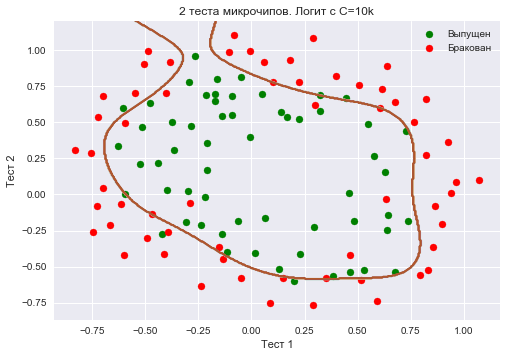
\includegraphics[scale=0.4]{images/test-06.png}
\end{figure}
Доля правильных ответов классификатора на обучающей выборке – 0.873.
\end{frame}

\begin{frame}[fragile]
Выводы:
\begin{itemize}
\item чем больше параметр $C$, тем более сложные зависимости в данных может восстанавливать модель;
\item если регуляризация слишком сильная (малые значения $C$), модель окажется недообученной (1 случай) и недостаточно "штрафуется" за ошибки;
\item если регуляризация слишком слабая (большие значения $C$), модель слишком "боится" ошибиться на объектах обучающей выборки, поэтому окажется переобученной (3 случай);
\item то, какое значение $C$ выбрать, сама логистическая регрессия "не поймет" (или еще говорят "не выучит"), то есть это не может быть определено решением оптимизационной задачи, которой является логистическая регрессия (в отличие от весов $w$). 
\end{itemize}
\end{frame}

\end{document}
